\documentclass[paper=a4, fontsize=11pt]{scrartcl}
\usepackage[T1]{fontenc}
\usepackage[polish]{babel}
\usepackage{multirow}
\usepackage{soul}
\usepackage[utf8]{inputenc}
\usepackage{fontspec}
\usepackage{graphicx}
\usepackage{amsmath}
\usepackage[export]{adjustbox}
\usepackage{float}
\usepackage{geometry}
\usepackage{gensymb}
\usepackage{listings}
\usepackage{indentfirst}
\usepackage[draft,nosingleletter]{impnattypo}
\begin{document}
	
	\begin{center}
		\begin{tabular}{cc}
			\hline
			\multicolumn{2}{|c|}{\begin{tabular}[c]{@{}c@{}} \\ \LARGE \so{Informatyka w Medycynie - Laboratorium} \\ \\ \end{tabular}}                                                                                                                                                                                                                  \\ \hline
			\multicolumn{2}{|c|}{\begin{tabular}[l]{@{}l@{}}\\\Large Tomografia komputerowa - projekt \\ \\ \end{tabular}}  \\ \hline
			\multicolumn{1}{|l|}{\begin{tabular}[l]{@{}l@{}} \\ \hspace{2cm}Kierunek/semestr: Informatyka/6 \hspace{2cm} \\ \\ \end{tabular}} &
			\multicolumn{1}{|c|}{\begin{tabular}[l]{@{}l@{}} \\ Grupa: L16 \\ \\ \end{tabular}}  \\ \hline
			\multicolumn{2}{|c|}{\begin{tabular}[c]{@{}c@{}}\\ Jakub Kwiatkowski 145356 \\Paweł Strzelczyk 145217  \\ \\ \end{tabular}}  \\ \hline
			
		\end{tabular}
	\end{center}

	\section{Opis projektu.}
	\section{Opis głównych funkcji programu.}
	\subsection{Pozyskiwanie odczytów dla poszczególnych detektorów.}
	\subsection{Filtrowanie sinogramu.}
	\subsection{Ustalanie jasności poszczególnych punktów obrazu wynikowego oraz jego przetwarzanie końcowe.}
	\subsection{Wyznaczanie wartości miary RMSE.}
	\subsection{Odczyt i zapis plików DICOM.}
	
	\section{Wpływ poszczególnych parametrów na jakość obrazu wynikowego.}
	\subsection{Liczba detektorów.}
	
	Liczba detektorów jest zmieniana w przedziale $\left<90, 720 \right>$ z krokiem $90$.
	
	\begin{center}
		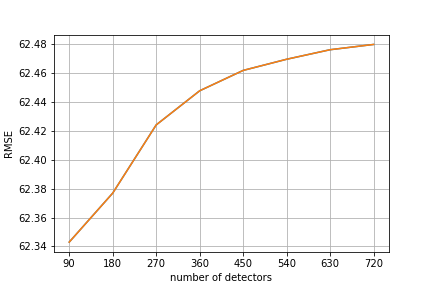
\includegraphics[width=0.7\textwidth]{detectors.png}
	\end{center}
	\subsection{Liczba skanów.}
	
	Liczba skanów jest zmieniana w przedziale $\left<90, 720 \right>$ z krokiem $90$.
	
	\begin{center}
		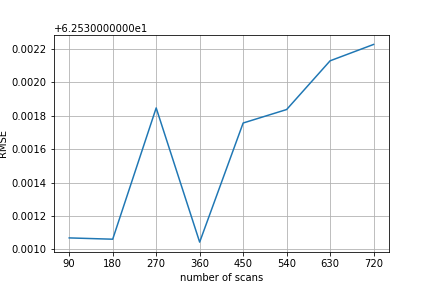
\includegraphics[width=0.7\textwidth]{scans.png}
	\end{center}
	\subsection{Rozpiętość wachlarza.}
	
	Rozpiętość wachlarza jest zmieniana w przedziale $\left<45, 270 \right>$ z krokiem $45$.
	
	\begin{center}
		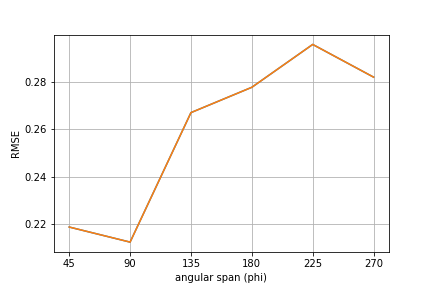
\includegraphics[width=0.7\textwidth]{phi.png}
	\end{center}
	\subsection{Filtr splotowy.}
	\begin{center}
		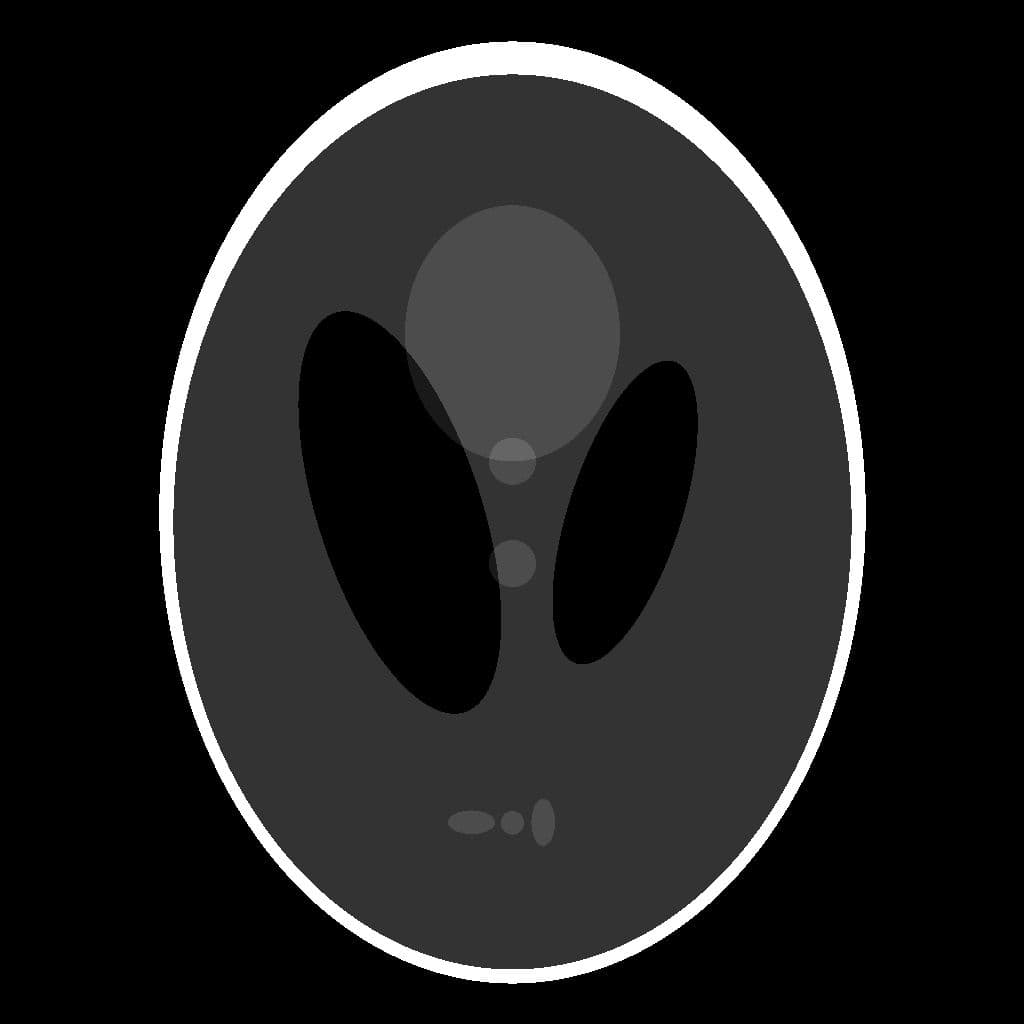
\includegraphics[width=0.8\textwidth]{phantom.png}
		
		
		Obraz testowy do obliczeń z wykorzystaniem filtra.
	\end{center}

	\begin{center}
		Rekonstrukcja bez filtrowania.
		
		
		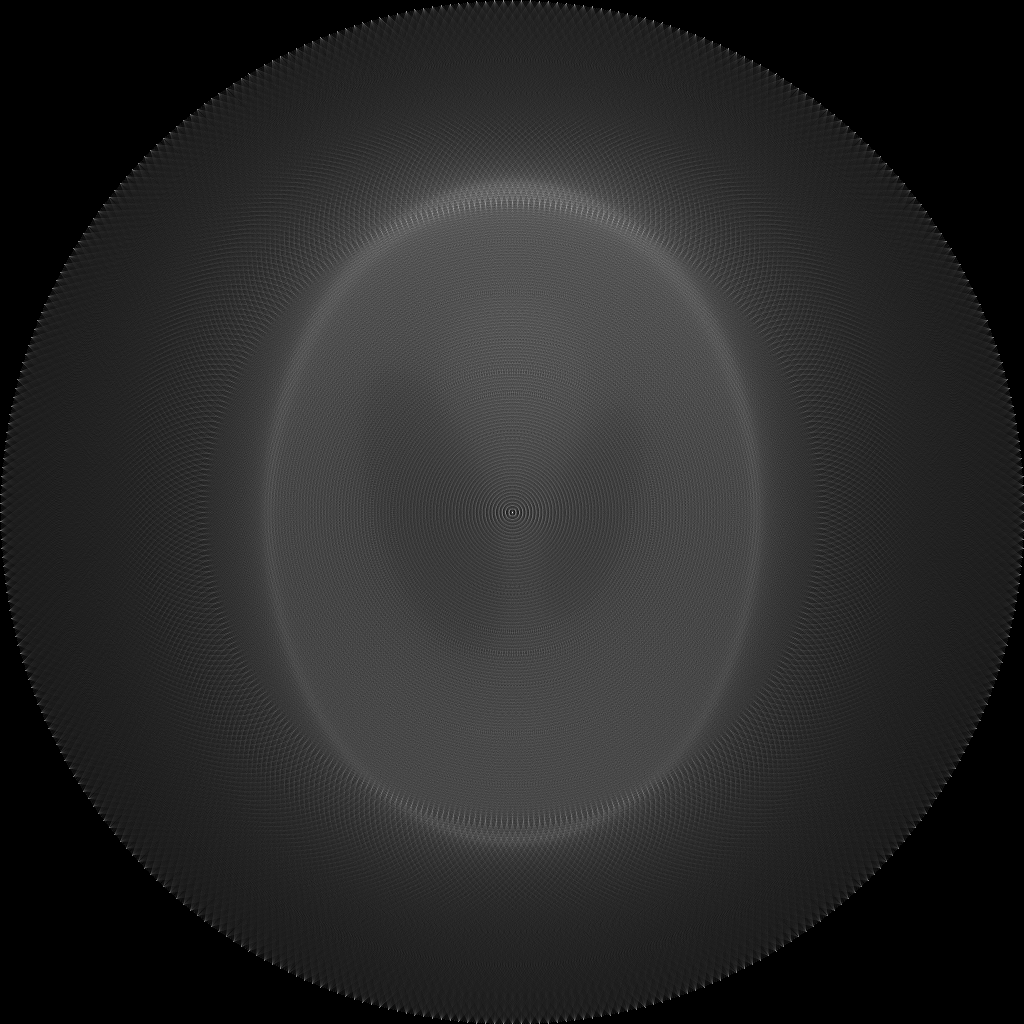
\includegraphics[width=0.4\textwidth]{reconstructed1.png}
		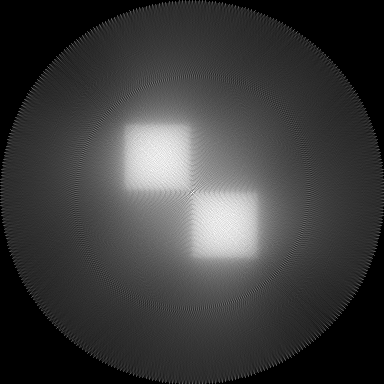
\includegraphics[width=0.4\textwidth]{reconstructed2.png}
		
		RMSE1 0,20693420547948 \hspace{1.5cm} RMSE2 0,266156126913852
		
	\end{center}
	
	
		\begin{center}
		Rekonstrukcja z filtrem.
		
		
		
\includegraphics[width=0.4\textwidth]{reconstructed_filtered1.png}
		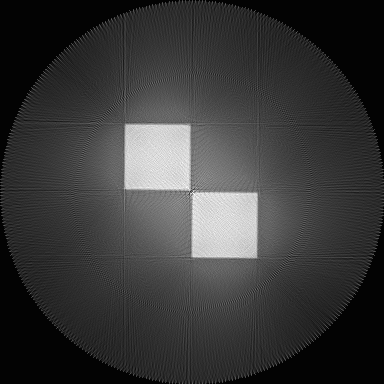
\includegraphics[width=0.4\textwidth]{reconstructed_filtered2.png}
		
		RMSE1 filtr - 0,249729691096470\hspace{1.5cm} RMSE2 filtr - 0,26778570956508
	\end{center}
	
	\section{Zmiana RMSE podczas wykonywania kolejnych iteracji odwrotnej transformaty Radona.}
	
	
	Parametry transformacji:
	\begin{itemize}
		\item liczba detektorów - 180
		\item rozpiętość wachlarza - 180\degree
		\item łączna liczba skanów - 180
	\end{itemize}
	\begin{center}
		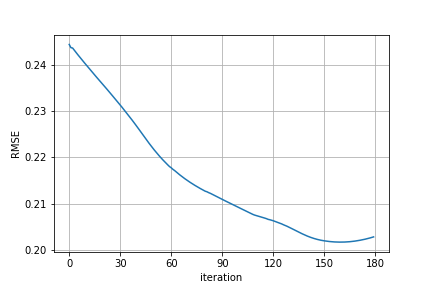
\includegraphics[width=0.7\textwidth]{change.png}
	\end{center}
\end{document}